%
% burgerintro.tex
%
% (c) 2018 Prof Dr Andreas Müller, Hochschule Rapperswil
%
\subsection{Nichtlineare Transportgleichung}
Die Gleichung von Burgers in der Form
\begin{equation}
\frac{\partial u}{\partial t} + u\frac{\partial u}{\partial x}=0
\qquad\text{mit Anfangsbedingung}\qquad
u(0,x) = u_0(x)
\label{burgers:transport}
\end{equation}
modelliert ein nichtlneares Transportproblem.
Die Gleichung~\eqref{burgers:transport} ist eine quasilineare partielle
Differentialgleichung erster Ordnung, die mit der Methode der
Charakteristiken \cite{burgers:pde} gelöst werden kann.
Die Charakteristiken-Gleichungen sind
\begin{align*}
t'(s)&=1
\\ 
x'(s)&=u
\\
u'(s)&=0
\end{align*}
Aus der ersten Gleichung leitet man ab, tdass $s=t$.
Die dritte Gleichung besagt, dass $u$ entlang einer Charakteristik konstant
ist, also $u(s)=u_0$.
Die zweite Gleichung besagt dann, dass die im Punkt $(0,x_0,u_0(x_0))$
beginnende Charakteristik eine Gerade mit $x(t)=x_0 + u_0(x_0)t$ ist.

\begin{figure}
\centering
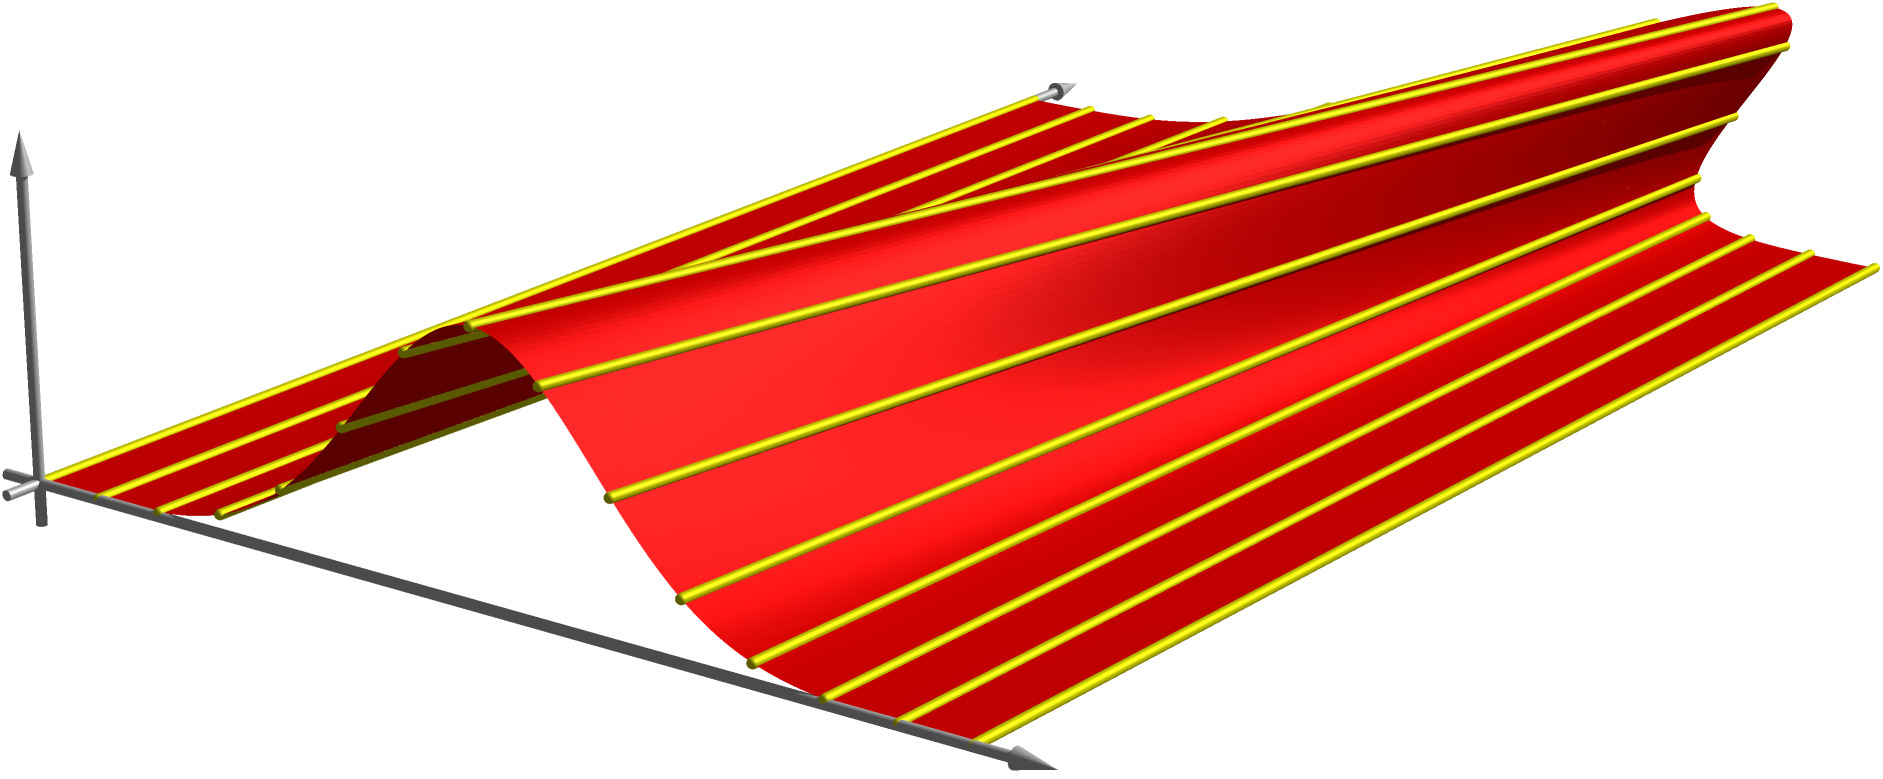
\includegraphics{learning/welle.jpg}
\caption{Lösung der Gleichung von Burgers
\label{burgers:charloesung}}
\end{figure}
Die Abbildung~\ref{burgers:charloesung} 
zeigt eine Lösung mit einer Gauss-Verteilung als Anfangsbedingung.
Es ist offensichtlich, dass die gezeigte Fläche früher oder später nicht
mehr Graph einer Funktion $u(x,y)$ sein kann.
Es entwickelt sich eine Sprungstelle, die Gleichung von Burgers ist
ein Modell für eine Schockwelle.
Man kann insbesondere nicht erwarten, dass die Gleichung von Burgers
für beliebige Zeiten $t$ eine glatte Lösung hat, selbst wenn die
Anfangsbedingungen glatt waren.
Man muss sich mit einer schwachen Lösung begnügen.
Dies hat sowohl auf numerische Lösungsverfahren Auswirkungen wie auch
auf das Problem, Trainingsdaten für auf Machine Learning basierenden
Lösungsalgorithmus zu erzeugen.

\subsection{Numerische Lösungen und Computational mode}
Bei der numerischen Lösung der Gleichung von Burgers tritt erschwerend der
Computational Mode auf.

